\chapter{Lösung}
Dieses Kapitel befasst sich mit den Möglichkeiten und den Lösungsansätzen, zu den Problemstellungen aus Kapitel \ref{ch:problem}. Anhand von Beispielen wird verdeutlicht, wie gewisse Anforderungen umgesetzt werden könnten.

\section{Meta-Modell}
Nach der Anforderungsanalyse, wurden alle relevanten Informationen erkannt und zusammen gestellt. Diese Zusammenstellung an Daten, welche die Applikation beschreiben wird \textit{Meta-Modell} genannt.

\subsection{Kompatibilität mit \acs{gemara} und andern möglichen Clients}

Um die Kompatibilität mit \acf{gemara} zu waren, wurde das \textit{Enfield-Meta-Modell} untersucht. Mit Hilfe dieser Untersuchung konnte festgestellt werden, an welcher Stelle zusätzliche Informationen für die \textit{Clients} am sinnvollsten eingebaut werden können. So das diese den Ablauf der Applikation gut beschreiben und an den benötigten Stellen alle relevanten Informationen für den Software-Generator zur Verfügung stellt.

Die Abbildung \ref{fig:enfield-model} zeigt die vereinfachte Modell-Klasse des \textit{Enfield-Meta-Modells}. 
In dieser Klasse sind bereits die wichtigsten Informationen wie zum Beispiel der Name der Applikation oder unter welchem \textit{Package} diese zu finden ist vorhanden. Neben diesen grundsätzlichen Informationen liefert die Modell-Klasse auch den Startpunkt des \textit{endlichen Automaten}, welcher die Anwendung beschreibt. Dieser Startpunkt ist der \textit{GetDispatcherState}. Dieses Objekt besitzt das Attribut \textit{transitions}. Dieses Attribut beschreibt, welche \textit{States} auf den \textit{Dispatcher-State folgen}. Jeder dieser folgenden \textit{States}, besitzt wiederum eine Collection mit \textit{Transitionen}, welche auf die nachfolgenden \textit{States} verweisen. So wird mit Hilfe der \textit{Transitionen} und der \textit{States} der \textit{endliche Automat} beschrieben. Der Generator kann diese Beschreibung nutzen, um zu entscheiden in welcher Reihenfolge, welche Klassen generiert werden müssen.

\begin{figure}[H]
	\begin{center}
		\includegraphics[width=0.86\textwidth]{images/Enfield-Meta-Model.png}
		\caption{Vereinfachter Aufbau des \textit{Enfield-Meta-Modells}.}
		\label{fig:enfield-model}
	\end{center}
\end{figure}

Um jetzt zusätzlich benötigten Informationen für die Android Applikation in dieses bestehende Modell einzubauen, gibt es zwei Möglichkeiten.

\subsection{Eigenes Android-Meta-Modell}

Es besteht die Möglichkeit die Modell-Klasse um ein Attribut \textit{Android-Meta-Modell} zu erweitern.
Die Abbildung \ref{fig:android-model} zeigt schemenhaft ein Beispiel wie ein \textit{Android-Meta-Modell} aussehen könnte. Auffällig hierbei ist, das viele Informationen, die das \textit{Enfield-Modell} bereits liefern würde, noch einmal explizit beschrieben werden müssen. Ein Beispiel wären die \textit{Transitionen}, zwischen den \textit{Fragmenten} beziehungsweise zwischen den \textit{Activities}. 


\begin{figure}[H]
	\begin{center}
		\includegraphics[width=0.86\textwidth]{images/Android-Meta-Model.png}
		\caption{Möglicher Aufbau eines \textit{Android-Meta-Modells}.}
		\label{fig:android-model}
	\end{center}
\end{figure}

Der Nutzer des Software-Generators, muss ziemlich viel über den Ablauf und die Funktionsweise einer Android-Anwendung wissen, um diesen Generator sinnvoll verwenden zu können.
Dabei bleibt zusätzlich noch die Möglichkeit, das der Nutzer eigens geschriebene Methoden in das Modell einpflegen kann. John Abou-Jaoudeh at al., haben in ihrer Arbeit \textit{A High-Level Modeling Language for Efficent Design, Implementation, and Testing of Android Applications}\cite{abou2015high} ein \textit{Meta-Modell} entwickelt, welches genau solche Features unterstützt.

Der Vorteil einer solchen Erweiterung des \textit{Enfield-Modell}s ist, das alle benötigten Daten für die Android Anwendung an einer Stelle zu finden sind. Auch hat der Nutzer die Möglichkeit an manchen Stellen eigene Methoden einzufügen und somit ist er in der Lage das Verhalten der App weiter zu individualisieren.

Jedoch überwiegen in diesem Fall die Nachteile. Ein Nachteil dieses Vorgehens ist, die redundante Beschreibung des Programm-Ablaufes. Einmal im \textit{Android-Meta-Modell} und einmal im \textit{Enfield-Meta-Modell}. Bei jeder Änderung gilt dies zu berücksichtigen. 
Der nächste Nachteil ist der, der Nutzer des Software-Generators muss sich in der Entwicklung von Android Anwendungen auskennen. Er muss genau das Zusammenspiel von \textit{ViewHoldern}, \textit{Adaptern}, \textit{Fragments} und \textit{Activities} kennen. Er muss wissen wie diese ineinandergreifen und wann welche Aktionen ausgelöst werden müssen. Weiterhin sollte er ein grundsätzliches Verständnis für das \textit{\acf{mvc} Pattern} besitzen, welches bei der Entwicklung von Android Applikationen Anwendung findet.
Ein weiterer Nachteil ist die Beschränkung des Modells auf Android. Wird das \textit{Enfield-Modell} um ein \textit{Android-Meta-Modell} erweitert, so muss dieses für jeden einzelnen \textit{Client} geschehen. Soll der Generator beispielsweise um Polymer-Webkomponente oder einer iOS-Anwendung erweitert werden, so müsste für jede einzelne Art von \textit{Client}, das \textit{Enfield-Modell} mit einem Entsprechenden \textit{Meta-Modell} erweitert werden.

\subsection{Allgemeine Erweiterungen des \textit{Enfield-Modell}s}

In dieser Arbeit wurde sich für die Variante entschieden, das \textit{Enfield-Modell} an geeigneter Stelle zu erweitern.
Diese Stelle befindet sich in den einzelnen \textit{States}. Jede Instanz des \textit{AbstractState} besitzt ein Attribut \textit{SingleResourceView}. Diese Klasse wird um die  Attribute, welche benötigt werden erweitert. In der Abbildung \ref{fig:enfield-model-extended} ist der vereinfachte Aufbau des \textit{AbstractStates} und einer \textit{SingleResourceView} zu sehen.

Wird beispielsweise eine Instanz eines \textit{GetPrimarySingleResourceByIdStates} erzeugt, und dessen \textit{SingleResourceView} enthält alle notwendigen Informationen, um die \textit{View} in der Android Anwendung zu beschreiben. Kann der Generator mit Hilfe der \textit{Transitionen} über die \textit{States} iterieren und verfügt an jedem \textit{State} über alle benötigten Informationen, um den aktuellen \textit{State} in der Anwendung generieren zu lassen.

\newpage

Bei dieser Methode befinden sich alle \textit{State}-spezifischen Daten direkt am \textit{State}. Jedoch gibt es neben diesen spezifischen Daten auch Daten, welche die komplette Applikation betreffen. Hierfür muss das \textit{Enfield-Modell} noch an einer andern Stelle erweitert werden. 
Es erscheint sinnvoll die Erweiterung direkt in der Modell-Klasse vorzunehmen. So kann der Generator schon am Anfang auf diese Daten zugreifen und diese verarbeiten.

Die Abbildung \ref{fig:enfield-model-extended} zeigt das \textit{Enfield-Modell}, welches um die oben genannten Informationen erweitert wurde.

\begin{figure}[H]
	\begin{center}
		\includegraphics[width=0.86\textwidth]{images/Enfield-Meta-Model-Erweitert.png}
		\caption{Vereinfachter Aufbau des erweiterten \textit{Enfield-Meta-Modells}.}
		\label{fig:enfield-model-extended}
	\end{center}
\end{figure}

Der Nachteil dieser Methode ist, das die Informationen an mehr als einer Stelle im \textit{Enfield-Modell} zu finden sind. Sollten die Informationen zu den \textit{Clients} verändert werden, so sind Änderungen an der \textit{SingleResourceView}-Klasse und in der Modell-Klasse nötig. Die Vorteile wurden jedoch oben schon einmal erwähnt. Der Generator kann das Modell als Fahrplan nutzen und weiß genau wann er welche Klassen für die Android Anwendung erzeugen muss. Er kann auch mit Hilfe der \textit{Transitionen} bestimmen wie der Verlauf innerhalb der Anwendung gestaltet ist.

\newpage
\subsection{Analyse der benötigten Dateien für das Meta-Modell}

Nachdem identifiziert wurde, an welchen Stellen das \textit{Enfield-Modell} erweitert werden soll, muss noch analysiert werden, welche Informationen an diesen Stellen zur Verfügung gestellt werden müssen. Bei dieser Analyse muss auch ein Augenmerk darauf gelegt werden, wie man die Informationen so aufbereitet, dass diese nicht nur eine Android-Applikation, sondern auch mögliche andere \textit{Clients} unterstützen.

Die Analyse in dieser Arbeit beschränken sich auf die \textit{Clients} Android und Polymer-Webkomponente. Bei beiden wird das \acf{ui} nach den Richtlinien,des von Google entwickelten Material Design, erstellt \cite{material}. Diese Richtlinien schreiben bereits viele nötigen Informationen für die Oberflächengestaltung vor. So wird beispielsweise definiert, das Einträge in einer Liste, als Karte dargestellt werden sollen. Abstände und Icons werden ebenfalls festgelegt.

\subsubsection{CardView}

\begin{figure}[H]
	\begin{center}
		
\includegraphics[width=0.86\textwidth]{images/card.png}
		\caption{Beispiel einer \textit{CardView} aus einer Liste von Dozenten nach Material Design.}
		\label{fig:card}
	\end{center}
\end{figure}

\newpage

\begin{lstlisting}[label=lst:braun_json,
language=json,
firstnumber=1,
caption=Demo Daten eines Dozenten.]	
...			   
{
	"address": "Sanderheinrichsleitenweg 20 97074 Wuerzburg",
	"chargeUrl": {
		"href": "https://apistaging.fiw.fhws.de/mig/api/lecturers/4/charges",
		"rel": "chargeUrl",
		"type": "application/vnd.fhws-charge.default+json"
	},
	"email": "peter.braun@fhws.de",
	"firstName": "Peter",
	"homepage": {
		"href": "http://www.welearn.de/.../prof-dr-peter-braun.html",
		"rel": "homepage",
		"type": "text/html"
	},
	"id": 4,
	"lastName": "Braun",
	"phone": "0931/3511-8971",
	"profileImageUrl": {
		"href":"https://apistaging.fiw.fhws.de/.../4/profileimage",
		"rel": "profileImageUrl",
		"type": "image/png"
	},
	"roomNumber": "I.3.27",
	"self": {
		"href": "https://apistaging.fiw.fhws.de/mig/api/lecturers/4",
		"rel": "self",
		"type": "application/vnd.fhws-lecturer.default+json"
	},
	"title": "Prof. Dr."
}
...
\end{lstlisting}

Die  \textit{\acf{json}} Repräsentation unter Listing \ref{lst:braun_json} beschreibt das Beispiel aus Abbildung \ref{fig:card}.
Jetzt gilt es zu überlegen, wie die Attribute des \ac{json} Objekts aufzubereiten sind, dass diese die Karte des Dozenten widerspiegeln. 
In erster Linie muss entschieden werden, welche der gelieferten Informationen sollen in der Liste für jeden einzelnen Dozenten angezeigt werden. Ist es sinnvoll Informationen zu gruppieren? Hier beispielsweise die Attribute \textit{firstName} und \textit{lastName}, diese sollen in einer Zeile angezeigt werden. Ist bekannt welche Informationen eine Karte enthalten soll, so muss auch noch die Reihenfolge der einzelnen Attribute auf Karte bestimmt werden.
Neben der Reihenfolge gibt es noch die Möglichkeit Schriftgröße oder Schriftfarbe der einzelnen Attribute unterschiedlich zu gestalten. Auch müssen die Standardicons den jeweiligen Attributen zuweisen werden. Es sollte weitergehend möglich sein einzelnen Attribute bestimmte Aktionen zuzuweisen. Beispielsweise beim Klick auf eine Homepage, sollte diese im Browser geöffnet werden, oder beim Klick auf die Adresse sollte die Applikation \textit{Maps} öffnen und die angeklickte Adresse dort anzeigen. Ein Attribut mit dem Hyperlink zu einer Website, sollte es möglich sein einen mitgegebenen Text anstelle des Hyperlinks anzuzeigen. 

Besitzt die Karte ein Bild, so sollte der Nutzer die Möglichkeit besitzen zu entscheiden ob dieses auf der linken oder rechten Seite der Karte dargestellt werden soll.

\subsubsection{DetailView}

\begin{figure}[H]
	\begin{center}
		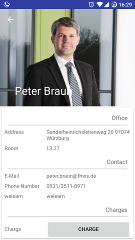
\includegraphics[width=0.4\textwidth]{images/detail.png}
		\caption{Beispiel einer \textit{DetailView} eines Dozenten nach Material Design.}
		\label{fig:detail}
	\end{center}
\end{figure}

Die zur Verfügung stehenden Daten sind die gleichen, welche unter Listing \ref{lst:braun_json} einzusehen sind.

Analog wie bei der \textit{CardView} stellt sich auch bei der \textit{DetailView} die Frage, welche Daten dargestellt werden sollen. Hier jedoch gibt es zusätzlich zu der horizontalen Gruppierung (Beispiel: Vornamen und Nachnamen), auch noch eine vertikale Gruppierung. Diese wird im weiteren auch Kategorisierung genannt. In der detaillierten Ansicht eines Dozenten gibt es die Möglichkeit Attribute zu kategorisieren und jeder Kategorie mit einem Namen zu versehen. Für die Gestaltung und Anordnung sowie mögliche Klick-Aktionen müssen die selben Anforderungen wie bei der \textit{CardView} berücksichtigt werden. 

Jedoch muss die \textit{DetailView} wissen, welches Attribut den Titel der \textit{View} darstellt, da dieser in der \textit{AppBar} erscheinen wird. In diesem Beispiel ist es der Name des Dozenten. Anders als bei der \textit{CardView} gibt es hier nicht die Möglichkeit zu bestimmen wo das Bild dargestellt werden soll. Ist ein Bild vorhanden, so wird dieses in der \textit{CollapsingToolbar} dargestellt \cite{collapsing}.
subsubsection{InputView}

\begin{figure}[H]
	\begin{center}
		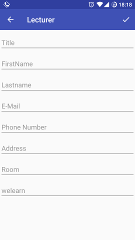
\includegraphics[width=0.4\textwidth]{images/input.png}
		\caption{Beispiel einer \textit{View} zum Anlegen eines Dozenten.}
		\label{fig:input}
	\end{center}
\end{figure}

Für das neu Anlegen eines Dozenten oder auch zum bearbeiten muss entschieden werden, welche Attribute zum Anlegen nötig sind. Auch hier ist es notwendig die Reihenfolge zu bestimmen. Jedoch kommen in dieser \textit{} für jedes Attribut noch die Möglichkeit hinzu ein \textit{Hint}-Text anzugeben. Dieser Text beschreibt, was in der Android \textit{View} \textit{EditText} als Beschreibung für das bestimmte Attribut steht. Weiter sollte es die Möglichkeit geben, jedem Feld eine Nachricht mitzugeben, welche angezeigt wird, wenn das Feld beispielsweise leer gelassen wird. Oder eine weitere Nachricht, wenn das Eingegebene nicht dem Erwarteten entspricht. Zum Beispiel wurde in das Feld für die E-Mail eine Telefonnummer eingegeben. Oder es wurde ein regulärer Ausdruck mitgegeben und das Eingegebene entspricht nicht dessen Anforderungen.

\subsubsection{Programmablauf und Klick-Aktionen}

Da das \textit{Enfield-Modell} bereits einen \textit{endlichen Automaten} beschreibt, welcher den Programmablauf widerspiegelt, ist es nicht notwendig, diesen Ablauf noch einmal genauer zu definieren. Der bereits definierte Ablauf übernommen wird.

Auch die Aktionen welche durch einen Klick auf ein bestimmtes Attribut ausgeführt werden soll, beschränkt sich auf Android Standardaktionen. Beispielsweise das wechseln zu den \textit{Maps}, zu einem \textit{E-Mail Client}, dem \textit{Browser} oder zum \textit{Anrufsmenü}. Jede dieser Aktion ergibt sich aus den Typen der Attribute, weswegen diese auch nicht weiter definiert werden müssen.

\subsection{Design der View-Meta-Modelle} \label{sec:resourceViews}

In den letzten Abschnitten der Arbeit wurde aufgezählt, was das \textit{Meta-Modell} sowohl Android- als auch Polymer-seitig abdecken muss. In diesem Kapitel wird ein \textit{Meta-Modell} vorgestellt, welches die erwähnten Eigenschaften abdeckt.


\begin{figure}[H]
	\begin{center}
		\includegraphics[width=\textwidth]{images/metamodel.png}
		\caption{Aufbau der \textit{Views} zur Erweiterung des \textit{Enfield-Modell}s.}
		\label{fig:meta-model}
	\end{center}
\end{figure}

Die Abbildung \ref{fig:meta-model} zeigt den Aufbau der Objekte, mit welchem das \textit{Enfield-Modell} erweitert wird. Die drei \textit{Views}: \textit{CardView}, \textit{DetailView} und \textit{InputView} sind alles Instanzen von \textit{AbstraktResourceView}. Jede der \textit{View}, weiß, durch die Zuordnung mit Hilfe des Ressourcennamens, welche Ressource sie darstellen soll. Die drei \textit{Views}, lassen sich in zwei Kategorien einteilen: \textit{Views}, welche Informationen anzeigen und \textit{Views} welche zur Eingabe von Informationen benötigt werden.
So gehören \textit{CardView} und \textit{DetailView} zu den anzeigenden \textit{Views} und die \textit{InputView} zur zweiten Kategorie. 

\subsubsection{Anzeigende Views}
Diese \textit{View}-Typen haben die Aufgabe eine Liste aller Attribute zu halten, welche in der entsprechenden \textit{View} angezeigt werden sollen. Dabei bestimmt die Reihenfolge, in welcher die Attribute in dieser Liste sind auch die Anordnung in der Oberfläche. Ist das erste Item in der Liste der Name, so wird dieser ganz oben in der \textit{View} angezeigt.
Bei der \textit{DetailView} jedoch gibt es nicht eine Liste mit den Attributen, sondern eine Liste mit Kategorien. Diese besitzen 
einen Namen und eine Liste mit den Attributen ihrer Kategorie. Die Darstellungsreihenfolge der Kategorien und deren Attribute ist analog zu der der \textit{CardView}. Weiter besitzt die \textit{DetailView} das Attribut \textit{image}, dieses wird hier aus der Liste der Attribute herausgezogen, da dieses Attribut bestimmt, ob die \textit{View} eine \textit{CollapsingToolbar} besitzen wird oder nicht. Wiederum haben beide \textit{Views} das Attribut \textit{titleOfResource} dieses bestimmt welches Attribut unserer Ressource beispielsweise in der \textit{Toolbar} angezeigt wird.

Auf die Polymer-spezifischen Attribute wird in dieser Arbeit nicht weiter eingegangen.

Mit Hilfe der Listen, Titelattributen und dem Bildattribut kann das Erscheinungsbild einer \textit{View} schon ziemlich gut beschrieben werden. Als nächstes wird auf Möglichkeit, Schriftgrößen, Schriftfarben und Klick-Aktionen zu definieren.
Außerdem ist es bis jetzt nur möglich einfache Attribute anzuzeigen, eine horizontale Gruppierung ist noch nicht möglich. Um diese Anforderungen zu erfüllen, werden nicht Attribute in den Listen gespeichert sondern Ausprägungen von \textit{ResourceViewAttributen}. 

Es gibt zwei Ausprägungsarten: \textit{SingleResourceViewAttribute} und \textit{GroupedResourceViewAttribute}.  Das \textit{SingleResourceViewAttribute} ist für einfache Attribute, mit diesem ist es beispielsweise möglich den Titel eines Dozenten anzuzeigen. Das \textit{GroupedresourceViewAttribute} ermöglicht die horizontale Gruppierung. Beide Objekte, bestimmen jedoch nicht die Design-spezifischen Eigenschaften des Attributs. Hierfür besitzen beide Attribut-Typen das Attribut \textit{DisplayViewAttribute}.

Bei der \textit{SingleResourceViewAttribute} ist diese Instanz von einem \textit{AbstractViewAttribute} das einzige Attribut, beim \textit{GroupedResourceViewAttribute} wiederum gibt es eine Liste von diesen \textit{DisplayViewAttributen}, welche dann die anzuzeigenden Informationen widerspiegeln. Weitergehend besitzt das \textit{GroupedResourceViewAttribute} auch noch ein \textit{DisplayViewAttribute}, welches die neu entstandene Gruppierung beschreiben soll.

Ein \textit{DisplayViewAttribute} besitzt nun die Möglichkeit, Schriftgröße und -farbe zu definieren. Die angegebene Farbe muss eine in hexadezimaler Darstellung angegeben werden, wird keine Farbe mitgegeben, wird die Defaultfarbe der Anwendung genommen. In der Regel ist diese Schwarz.  Die Schriftgröße wiederum ist auf 3 Stufen beschränkt. Es gibt die Möglichkeit den Text in klein, normal und groß darzustellen. Per default ist normal eingestellt. Aus der Oberklasse \textit{AbstractViewAttribute} besitzt das \textit{DisplayViewAttribute} noch die Attribute \textit{attributeName}, dieses muss exakt so heißen wie in der Definition der Ressource.
Mit dem \textit{attributeLabel} kann angegeben werden, wie dieses Attribut in der \textit{View} angezeigt werden soll. Die Abbildung \ref{fig:detail} zeigt die Verwendung von den Labels, vor beispielsweise der E-Mailadresse des Dozenten steht \textit{E-Mail}, dieser String entspricht dem Label des Attributes. Weiterhin muss angeben werden von welchem Typ das aktuell beschriebene Attribut ist.
Dies geschickt mit dem Attribut \textit{AttributeType}. Es gibt folgende mögliche Typen: \textit{HOME}, \textit{MAIL}, \textit{LOCATION}, \textit{PICTURE}, \textit{PHONE\_NUMBER}, \textit{TEXT}, \textit{URL}, \textit{DATE}, \textit{SUBRESOURCE}. Jeder Typ bestimmt die Eigenschaften des Attributes. Über diesen wird bestimmt welches Icon in der Karte vor dem entsprechenden Attribut angezeigt wird oder welche Aktion bei Klick ausgeführt werden soll. So wird bei einem Klick auf ein Attribut vom Typ \textit{LOCATION} versucht die Anwendung \textit{Maps} zu öffnen und den angezeigten Standort dort anzuzeigen. Ist das Attribute vom Typ \textit{SUBRESOURCE} so wird für dieses Attribut ein \textit{Button} angezeigt, dieser ermöglicht es dann zu der entsprechenden Subressource zu wechseln. Diese Klick-Aktionen müssen jedoch mit dem Attribut \textit{clickActionAndroid} erst aktiviert werden.
Manche Typen bringen noch ein paar andere Besonderheiten mit sich. So muss man beispielsweise bei einem \textit{URL}-Attribut noch eine Beschreibung mitgeben, welche anstelle der Hyperlinks angezeigt werden soll. Bei einem Bild kann beispielsweise noch bestimmt werden, ob dieses links oder rechts dargestellt werden soll. 

Das im Anhang befindliche Listing \ref{lst:detailview_impl} zeigt die Definition einer \textit{DetailView}.

\subsubsection{Eingebende Views}

Bei der \textit{InputView} gibt es wieder eine Liste, welche dieses mal \textit{InputViewAttribute} mit der Oberklasse \textit{AbstractViewAttribute} hält. Diese Liste bestimmt analog zu den anzeigenden Views die darzustellende Reihenfolge der Attribute. 

Neben dem \textit{attributeName} der wieder exakt dem Namen aus der Ressourcendefinition entsprechen muss, besitzt das \textit{InputViewAttribute} auch die Möglichkeit zu bestimmen, welcher Typ das aktuelle Attribut besitzt. Jedoch haben die Typen hier eine andere Bedeutung als bei dem anderen \textit{View}-Typ. So wird beispielsweise bei dem Type \textit{DATE} kein \textit{EditText} angezeigt, sondern der Nutzer hat die Möglichkeit das Datum über das \textit{DatePicker-Widget} von Android einzugeben. 

Es ist jedoch für den Android-\textit{Client} nicht möglich Bilder zu Ressourcen hinzuzufügen, oder diese zu Bearbeiten. Des weiteren wird eine Subressource nicht in einer \textit{InputView} der Oberressource bearbeitet oder neu angelegt. Dies geschieht in der entsprechenden \textit{View} der Subressource. Die anderen Typen beschränken das \textit{EditText-Widget} auf die angegebenen Typen. So wird beispielsweise bei einem Klick auf ein \textit{PHONE\_NUMBER-Feld} die Tastatur im Zahlenmodus ausgefahren.

Einem \textit{InputViewAttribute} muss zusätzlich ein \textit{hintText} mitgegeben werden, der im \textit{EditText} des Attributs beschreibt, was in diesem Feld erwartet wird. Mit dem String \textit{missingText} kann dem Attribut mitgegeben werden, welche Nachricht dem Nutzer angezeigt wird, falls er versucht zu speichern ohne das entsprechende Feld auszufüllen. Mit der Kombination von \textit{checkPattern} und \textit{errorText} bekommt der Nutzer des Generators die Möglichkeit die Validierung des eingegebenen Attributes noch weiter zu verfeinern und auch dem Nutzer der Applikation ein Feedback zu geben, falls eine falsche Eingabe getätigt wurde.

Die Definition einer \textit{InputView} wird im Anhang unter Listing \ref{lst:inputview_impl} dargestellt.

\subsection{Analyse und Design von allgemeinen Daten für eine Anwendung}

Dieses Kapitel behandelt die Informationen, welche eine Applikation neben den \textit{View}-Beschreibungen zusätzlich benötigt, aber diese vom Kontext her nicht in einer der \textit{Views} beschrieben werden können.

Ein Beispiel für eine solche Information wäre der \acf{url} für den Einstieg. Die Applikation benötigt diesen um zu wissen, unter welcher Adresse die anzuzeigenden Informationen zu finden sind. Ein weiteres Beispiel sind die Grundfarben der Applikation. Das Material Design gibt drei benötigte Grundfarben vor: \textit{colorPrimary}, \textit{colorprimaryDark} und \textit{colorAccent} diese Grundfarben werden um die Farbe für den \textit{Toolbar}-Text erweitert.

Mit dem Wissen, konnte eine Erweiterung des \textit{Enfield-Modell}s designet werden, welches in Abbildung \ref{fig:appspecifics} dargestellt ist.

\begin{figure}[H]
	\begin{center}
		\includegraphics[width=0.86\textwidth]{images/appspecifics.png}
		\caption{Aufbau des \textit{AppSpecifics} Objekt  zur Erweiterung des \textit{Enfield-Modell}s.}
		\label{fig:appspecifics}
	\end{center}
\end{figure}

 Über die \textit{Map} \textit{additionalInformation} können zusätzlich weitere allgemeine Informationen an den Generator, weitergegeben werden.

\section{Software-Generator}

Dieses Kapitel behandelt die Funktionsweise und den Aufbau des Generators. Des weiteren wird das Java \acf{api} \textit{JavaPoet} kurz vorgestellt \cite{poet}.

\subsection{JavaPoet}
\textit{JavaPoet} ist ein Java \textit{\ac{api}}, welches ermöglicht Java-Klassen zu generieren \cite{poet}. Hierfür wird die zu generierende Klasse programmiert. Mit Hilfe von nur ein paar Schlüsselwörtern ist es möglich \textit{Klassen}, \textit{Interfaces} oder \textit{Methoden} zu generieren. 

Da der größte Teil des Generators Java-Klassen erzeugen muss, ist dieses \ac{api} bestens für diesen Zweck geeignet. Sie erspart die aufwändige String-Manipulation. Durch die Nutzung wird auch bei der Ausführung des Programmes sichergestellt, das gültige Konventionen und Regeln von Java eingehalten werden. So ist der grundsätzliche korrekte Aufbau einer Java-Klasse bereits vorab sichergestellt.

Listing \ref{lst:poet} zeigt ein einfaches Beispiel zur Generierung einer Hello-World-Klasse und Listing \ref{lst:poet_result} zeigt das Ergebnis nach der Ausführung des Beispieles.

\begin{lstlisting}[label=lst:poet,
language=java,
firstnumber=1,
caption=Beispiel für die Generation einer Hallo-World-Klasse \cite{poet}.]				   
MethodSpec main = MethodSpec.methodBuilder("main")
	.addModifiers(Modifier.PUBLIC, Modifier.STATIC)
	.returns(void.class)
	.addParameter(String[].class, "args")
	.addStatement("$T.out.println($S)", System.class, "Hello, JavaPoet!")
	.build();

TypeSpec helloWorld = TypeSpec.classBuilder("HelloWorld")
	.addModifiers(Modifier.PUBLIC, Modifier.FINAL)
	.addMethod(main)
	.build();

JavaFile javaFile = JavaFile.builder("com.example.helloworld", helloWorld)
	.build();
\end{lstlisting}

\begin{lstlisting}[label=lst:poet_result,
language=java,
firstnumber=1,
caption=Ergebnis der Generation von Listing \ref{lst:poet} \cite{poet}.]				   
package com.example.helloworld;

public final class HelloWorld {
	public static void main(String[] args) {
		System.out.println("Hello, JavaPoet!");
	}
}
\end{lstlisting}

\subsection{Generierung anderer Daten-Typen}

Neben Java-Klassen besitzt der Quellcode einer Android Applikation auch \textit{XML}-Dateien und \textit{Gradle}-Dateien. Für diese Typen muss eine andere Möglichkeit der Generierung gewählt werden. Hierfür liefert \acf{gemara} mit der Klasse \textit{GeneratedFile} eine Möglichkeit. Diese Klasse besitzt die beiden Methoden \textit{append(String contet)} und \textit{appendln(String content)}. Welche es ermöglichen jedes beliebige textbasiertes File-Format zu generieren. Ein \textit{GeneratedFile} Objekt erzeugt eine Datei, welcher mit den beiden erwähnten Methoden Strings hinzugefügt werden können. Dies ermöglicht es jede beliebige Textstruktur zu erzeugen. Jedoch liefert diese Klasse keinerlei Validierung, die Datei wird generiert egal ob die Struktur gültig ist oder nicht.

Listing \ref{lst:append} erzeugt eine in Listing \ref{lst:append_result} dargestellte Datei \textit{test.xml} unter dem Verzeichnis \textit{generated}.
\begin{lstlisting}[label=lst:append,
language=java,
firstnumber=1,
caption=Beispiel eine \textit{GeneratedFile}-Instanz zur Erzeugung einer \textit{XML}-Datei.]				   
public class FileGenerator extends GeneratedFile {

	@Override
	public void generate() {
		appendln("<?xml version=\"1.0\" encoding=\"utf-8\"?>");
		appendln("<menu xmlns:android=\"http://schemas.android.com/apk/res/android\" xmlns:app=\"http://schemas.android.com/apk/res-auto\">");
		appendln("<item android:id=\"@+id/saveItem\"");
		appendln("android:title=\"@string/save\"");
		appendln("app:showAsAction=\"always\"\\>");
		appendln("<\\menu>");
	}

	@Override
	protected String getFileName() {
		return "test.xml";
	}

	@Override
	protected String getDirectoryName() {
		return "/generated";
	}
}
\end{lstlisting}

\newpage

\begin{lstlisting}[label=lst:append_result,
language=xml,
firstnumber=1,
caption=Erzeugte \textit{XML}-Datei durch den Quellcode von Listing \ref{lst:append}.]				   
<?xml version="1.0" encoding="utf-8"?>
	<menu xmlns:android="http://schemas.android.com/apk/res/android"
		xmlns:app="http://schemas.android.com/apk/res-auto">
		<item android:id="@+id/saveItem"
			android:title="@string/save"
			android:icon="@drawable/ic_done"
			app:showAsAction="always"/>
	</menu>
\end{lstlisting}

\subsection{Aufbau der zu generierenden Applikation}
Um eine Android Applikation generieren zulassen müssen nicht alle Klassen, generiert werden. Es können auch Überlegungen angestrebt werden, generischen Klassen einfach im Generator abzulegen und bei Bedarf zu kopieren. Diese Methode wurde verworfen, da andernfalls jedes mal die kopierten Klassen via String-Manipulation bearbeitet werden müssten. Die minimale Änderung welche jedes mal getroffen werden müsste, wäre das Anpassen der \textit{Package} Anweisung am Anfang der Java-Klassen und die der \textit{Import}-Anweisungen. Eine weitere Überlegung wäre es, diese Klassen in eine Android Bibliothek auszulagern, und diese dann in jede Anwendung zu importieren. Auch von dieser Möglichkeit wurde in der ersten Version abgesehen, da die Applikation bereits aus zwei Komponenten besteht. Der Applikation an sich und einer Bibliothek, welche die Android-Komponenten für die Anwendung enthält. Um die Komplexität zu reduzieren werden die benötigten generischen Klassen als Teil der eingebunden Bibliothek jedes mal aufs neue generiert.

%todo problem mit bild aus dem anhang
Der Aufbau und der Funktionsumfang der Referenzimplementierung wird in Kapitel \ref{sec:ref_impl} vorgestellt. Das Schaubild \ref{fig:lecturer_structure} aus dem Anhang verdeutlicht das Verhältnis von generischen (weiße Kästen) und spezifischen (rote Kästen) Klassen. Die Anzahl der gleichbleibenden Klassen ist mit etwa 60 Prozent bereits höher als der Anteil an spezifischen Klassen. Je höher der Anteil dieser unveränderlichen Klassen, desto geringer wird die Komplexität des Generators. Da der Aufwand eine spezifische Klasse zu erzeugen mehr Logik benötigt, als eine Klasse, welche immer gleich bleibt.

Daneben zeigt die Abbildung, auch noch die Aufteilung der Klassen in Klassen der Applikation (gestrichelte Kästen) und Klassen der Bibliothek (solide Kästen). Die Applikation an sich besteht nur aus ein paar wenigen \textit{Fragmenten} und \textit{Aktivities}, welche alle projektspezifisch sind. Der komplette generische Quellcode befindet sich in der Bibliothek. Des weiteren befinden sich dort auch die spezifischen Komponenten, beispielsweise der \textit{LecturerInputView}. Diese Komponente, kann in den Fragmenten zur Bearbeitung oder Neuanlage eines Dozenten dann mit wenigen Zeilen Programmcode verwendet werden.

Diese Art der Aufteilung ermöglicht es das ein Applikation Entwickler sich die Komponente, für das Anzeigen, Bearbeiten, Löschen und der Neuanlage generieren lassen kann. Diese Komponenten jedoch beliebig in seiner eigenen Applikation verwenden kann.

\subsection{Aufbau des Generators}

\begin{figure}[H]
	\begin{center}
		\includegraphics[width=\textwidth]{images/Welling.png}
		\caption{Aufbau des Android-Generators Welling.}
		\label{fig:welling}
	\end{center}
\end{figure}


Die Klasse \textit{ApplicationGenerator}, ist der Einstiegspunkt des Projekts. Sie erwartet im Konstruktor ein \textit{Enfield-Modell} Objekt. Wie der Abbildung \ref{fig:welling} entnommen werden kann, so lässt sich das Projekt in drei Teilbereiche gliedern. Der erste Bereich erzeugt ein \textit{AppDescription} Objekt (Abbildung \ref{fig:appDescription}) der zweite Bereich befasst sich mit allgemeinen Vorbereitungen, die getroffen werden müssen. Der Letzte iteriert über die \textit{States}, und generiert nach Bedarf die benötigten Klassen.

Die \textit{ApplicationGenerator} Klasse verfügt über eine öffentliche Methode \textit{generate}. Beim Aufrufen dieser Methode, werden die einzelnen Generatoren, für den allgemeinen Bereich angestoßen. Weiterhin wird das iterieren über die \textit{States} des \textit{Enfield-Modell} begonnen. Zum Schluss wird noch das \textit{AppDescription} Objekt ausgewertet, und die darin enthaltenen Informationen in Dateien geschrieben und an die entsprechende Stelle im Projekt gespeichert.

\subsubsection{Erstellung der AppDescription}

\begin{figure}[H]
	\begin{center}
		\includegraphics[width=\textwidth]{images/AppDescription.png}
		\caption{Aufbau des \textit{AppDescription} Objekts.}
		\label{fig:appDescription}
	\end{center}
\end{figure}

In der \textit{AppDescription} werden alle allgemeinen Daten durch den Generator gereicht, welche an vielen Stellen benötigt werden. 
Zum Beispiel der Name der Anwendung oder der Bibliothek. In jeder Java-Klasse wird der Paketname benötigt, da dieser in der Bibliothek und in der normalen Applikation verschieden sind, müssen diese für beide mitgeführt werden. Auch muss der Generator wissen, unter welchen Verzeichnissen die aktuelle Datei egal ob Java Klasse oder \textit{XML}-Datei gespeichert werden soll. 
Diese Informationen können einfach aus dem \textit{Enfield-Modell} abgelesen werden. Auch die Ressourcen und die jeweiligen Subressourcen können direkt aus dem \textit{Meta-Modell} entnommen werden.  Dies ist der Teil des initialisieren der \textit{AppDescription}. Alle bereits verfügbaren Informationen werden der \textit{AppDescription} zugewiesen. 

\newpage

Neben diesen Daten, die an mehreren Stellen bei der Generierung benötigt werden, gibt es Dateien in einer Android-Applikation, die sich mit dem Generieren aufbauen. Ein Beispiel für eine solche Datei ist die \textit{strings.xml}. 
Es wird in dem generierten Projekt zwei davon geben. Eine im Bereich der Applikation selbst und eine weitere in der Bibliothek. Diese Dateien enthalten neben dem Applikationsnamen beziehungsweise des Bibliotheksnamen auch viele Strings, die erst beispielsweise in einem Fragment auftauchen. Jedoch müssen die benötigten Datensätze in der \textit{strings.xml} eingetragen werden. Anstelle dies jedes mal wenn im Ablauf des Generierens ein String auftaucht, eine bereits generierte Datei zu erweitern, wird der Datensatz in der \textit{AppDescription} unter dem \textit{AppString} \textit{appString} beziehungsweise dem \textit{AppString} \textit{libString} hinterlegt.

Auch das \textit{AndroidManifest} wächst mit der Anwendung. So muss jede benutzte \textit{Aktivity} dort eingetragen sein. Andernfalls kann diese nicht genutzt werden. Am Anfang des Generierens ist die genaue Anzahl und die genauen Namen der \textit{Aktivities} unbekannt, weswegen der Generator diese beim Erzeugen zur \textit{AppDescription} hinzufügen muss. 
Das Attribut \textit{appDeclareStyleable} enthält alle \textit{CustomViews}, welche wie, im Kapitel \ref{sec:custom_view}, in die \textit{attr.xml} eingetragen werden müssen.

Da die Anwendung, welche generiert wird auch den \acf{rest} Ansätzen entsprechen soll, muss diese wissen welche \textit{Relationstypen} zu welchen Endpunkten gehören. Anfangs sind diese jedoch ebenfalls unbekannt und werden erst im weiteren Verlauf beim iterieren über die \textit{States} bekannt und zur \textit{AppDescription} hinzugefügt.
So wächst die \textit{AppDescription} über den gesamten Prozess des Generierens. Am Ende, werden die gesammelten Daten in die entsprechenden Dateien an den jeweiligen Orten gespeichert. Das Verwenden und weiterreichen eines \textit{AppDescription} Objekts reduziert die Komplexität des Generators. Dieser muss nicht bei jeder Ergänzung einer der beschriebenen Dateien diese Aufrufen, den neuen Datensatz aufwändig hinzufügen und die Datei wieder abspeichern. Sondern der Generator muss die Datei nur einmal schreiben, da er zum Beginn des Schreibvorgangs alle von der Android Anwendung benötigten Informationen besitzt.

\subsubsection{Vorbereitung und Generierung allgemeiner Dateien}

Der Bereich zur Vorbereitung und Generierung der allgemeinen Dateien gliedert sich ebenfalls in drei Bereiche. Der erste Bereich kümmert sich um alle Dateien die von \textit{Gradle} benötigt werden. 

Er kopiert Daten wie die \textit{gradlew.bat}, \textit{gradlew}, \textit{build.gradle} und den \textit{Gradle Wrapper}. 
Neben dem Kopieren, werden sowohl für die Applikation, Bibliothek als auch für das Gesamtprojekt die spezifischen Dateien generiert. So wird beispielsweise auf der Projektebene eine \textit{settings.gradle} erzeugt oder in der Applikation sowie der Bibliothek jeweils eine \textit{build.gradle}.

In der Sektion der Vorbereitung für die Applikation, werden Dateien erzeugt, die jede Applikation benötigt unabhängig von ihrem Aufbau oder den Features. Es wird beispielsweise die \textit{MainActivity} erzeugt, oder die \textit{XML}-Dateien, welche für die \textit{Transitions-Animationen} verantwortlich sind. Auch die \textit{styles.xml} wird erzeugt. Am Schluss werden noch die \textit{mipmap}-Ordner an dir richtige Stelle kopiert.

%ref{fig:lecturer}
Der Bereich, welcher die Bibliothek initialisiert, ist der Größte. Er generiert alle generell benötigten Klassen. Darunter fallen die Klassen der Netzwerkkommunikation, die Klasse für das Link-Objekt sowie das Interface \textit{Resource}. Es werden des weiteren auch die größten Teile der in der Abbildung \ref{fig:lecturer} abgebildeten generischen Klassen erzeugt. Auch werden die grundsätzlichen \textit{CustomViews} bereits erzeugt. Dazu gehören auch die benötigten \textit{XML}-Dateien. So kann für die Bibliothek beispielsweise das Manifest bereits erzeugt werden, da hier keine \textit{Activities} registriert werden müssen. Nach dem Ausführen des \textit{PrepareLibGenerators} steht, das Grundgerüst der Bibliothek. Diese enthält nun alle bereits vorab erzeugbaren und benötigten Dateien, welche unabhängig von der gewünschten Funktion der Applikation benötigt werden. 

Dieser gesamte Teilbereich des Projekts befasst sich damit ein Grundgerüst für die komplette Android Applikation zu erzeugen und vorab bereits alle benötigten Dateien aufzubereiten. Die generierten Klassen haben jedoch noch keinerlei Programmlogik, die den spezifischen Ablauf der zu generierenden Anwendung steuert.

\subsubsection{Iterieren über die States}

Der Teilbereich, der sich mit dem iterieren über die einzelnen \textit{States} beschäftigt ist der komplexeste Bereich des Generators. Er ist dafür verantwortlich, das zu jedem \textit{State} die alle benötigten Klassen und Dateien generiert werden. 

Um diese Anforderung zu erfüllen, nutzt er den \textit{Visitor} \textit{IStateVisitor}, welcher durch das \textit{Enfield-Modell} zur Verfügung gestellt wird. Außerdem wird auch der \textit{Visitor} \textit{VisitStatesOnlyOnce} benutzt. Dieser zweite \textit{Visitor} stellt sicher, das jeder \textit{State} nur einmalig besucht wird. Würde der Generator einfach nur über die Transitionen der \textit{States} gehen, könnte es passieren, das er in eine Endlosschleife endet.

Gelangt der Generator zu einem \textit{State}, wird mit dem \textit{ISateVisitor} identifiziert, von welchem Typ dieser ist. Mögliche \textit{Statetypen} sind: ein \textit{State} welcher einen \textit{GET-Request} auf eine einzelne Ressource oder auf eine Collection beschreibt oder \textit{States} welche einen \textit{POST-}, \textit{PUT-} oder \textit{DELETE-Request} repräsentieren.  Nach dieser Identifikation, wird bei jedem \textit{State}, außer dem \textit{DELETE-State}, eine Klasse für die in diesem \textit{State} betroffene Ressource erzeugt. Hierfür wird der \textit{ResourceGenerator} benutzt. Auch wenn dabei die Ressource mehrfach angelegt werden würde. Der Generator überschreibt eine bereits angelegte Ressource. Diese Redundanz garantiert das auf jeden Fall eine Ressource zum betreffenden \textit{State} existiert. 

Neben diesen Ressource-Klassen, wird auch ein \textit{StateHolder}-Objekt erstellt. Die Abbildung \ref{fig:stateHolder} repräsentiert dieses. 

\begin{figure}[H]
	\begin{center}
		\includegraphics[width=0.3\textwidth]{images/StateHolder.png}
		\caption{Aufbau des \textit{StateHolder} Objekts.}
		\label{fig:stateHolder}
	\end{center}
\end{figure}

Dieses Objekt wird für jeden einzelnen \textit{State} angelegt, es enthält alle \textit{States}, welche über die \textit{Transitionen} erreicht werden können.
So weiß der Generator genau, ob beispielsweise ein \textit{Button} angezeigt werden muss, der eine Neuanlage einer Ressource ermöglicht. Diese Informationen stecken zwar auch im \textit{Enfield-Modell}, jedoch müsste jedes mal wenn überprüft werden soll welche \textit{Folgestates} ein \textit{State} besitzt, über alle \textit{States} iteriert werden. Das \textit{StateHolder}-Objekt beschreibt sozusagen eine Landkarte für jeden einzelnen \textit{State}.

Der \textit{State}, welcher für das Löschen einer Ressource verantwortlich ist, ist der einfachste zum generieren. Hierfür wird lediglich ein \textit{DialogFragment} erzeugt, welches für das Löschen verwendet wird. 

Für die anderen \textit{States}, werden mehr Klassen und Dateien benötigt. Außerdem werden die \textit{ResourceViews} (Kapitel \ref{sec:resourceViews}) benötigt, die jedem \textit{State} angehängt sind. Zur Identifizierung der einzelnen \textit{ResourceViews} wird wiederum mit dem \textit{Visitor-Pattern} gearbeitet. Die Klasse der \textit{ResourceView} stellt den \textit{Visitor} \textit{ResoruceViewVisitor} zur Verfügung. 
Nachdem bekannt ist welche der drei \textit{ResourceView}-Typen im entsprechenden \textit{State} verwendet wurde, kann einer der Komponentengeneratoren: \textit{InputViewGenerator}, \textit{CardViewGenerator} oder \textit{DetailViewGenerator} alle notwendigen Dateien generieren.

\begin{figure}[H]
	\begin{center}
		\includegraphics[width=\textwidth]{images/Lecturer-Swimlines.png}
		\caption{Aufbau der Dozenten Applikation mit Einteilung in spezifische \textit{States}.}
		\label{fig:swimlines}
	\end{center}
\end{figure}

In Abbildung \ref{fig:swimlines} ist die Applikation für Dozenten noch einmal abgebildet. Zur Vereinfachung wurde bei diesem Diagramm jedoch die Ressource Ämter mit ihren zugehörigen Klassen weggelassen.

Der Bereich \textit{Update} und der Bereich \textit{Create} werden hierbei vom \textit{InputViewGenerator}, der Bereich \textit{Read Collection} von \textit{CardViewGenerator} und der Bereich \textit{Read Single} vom \textit{DetailViewGenerator} erzeugt.
Jeder der einzelnen Generatoren ist ein Zusammenschluss von vielen Teilgeneratoren. Es werden dabei in einem der Generatoren nicht nur die Java-Klassen für Applikation oder Bibliothek, sondern auch alle benötigten \textit{XML}-Dateien erzeugt.

\newpage

So ist beispielsweise der \textit{DetailViewGenerator} dafür verantwortlich, dass auf Seite der Applikation, die \textit{LecturerDetailActivity} inklusive ihrer XML-Datei erzeugt wird. Er muss weitergehend auch diese \textit{Aktivity} in die \textit{AppDescription} im Bereich des \textit{Manifestes} hinterlegen. Im Bereich der Bibliothek muss dafür gesorgt werden, dass die generischen Klassen \textit{ResourceDetailActivity}, \textit{ResourceDetailView} sowie die spezifischen Klassen: \textit{LectuererDetailView}, \textit{LectuererDetailAdapter}, \textit{LectuererDetailViewHolder}, \textit{LectuererDetailCardView} erzeugt werden. Zu all diesen Klassen müssen mögliche Strings oder \textit{CustomViews} in die \textit{AppDescription} aufgenommen werden. Wiederum müssen auch die entsprechenden \textit{XML}-Dateien erzeugt werden. 

Jeder Generator besitzt mehrere Möglichkeiten, welche Klassen generiert werden müssen. So entscheidet beispielsweise ob die Ressource ein Bild besitzt oder nicht über den Verhalt, ob eine \textit{Activity} mit einer \textit{CollapsingToolbar} verwendet wird oder ob ein einfaches \textit{Fragment} zur Detailanzeige ausreichend ist.
Selbst die Generatoren auf der untersten Ebene, welche die einzelne Klassen erzeugen, wissen mit Hilfe von dem mitgegebenen \textit{StateHolder}, ob beispielsweise Menüeinträge für das Löschen oder das Bearbeiten von Ressourcen benötigt werden. Diese Generatoren richten sich auch nach den übergebenen \textit{RessourceViews}. Auf dieser Ebene haben die vom Benutzer des Generators mitgegebenen Informationen zum Aussehen, Einfluss. Hier werden die benötigten Attribute der Ressource hinzugefügt, und deren Aussehen in den entsprechenden \textit{XML}-Dateien beschrieben.


\section{Bauen und ausführen der generierten Android Applikation}

Wurden alle benötigten Dateien der Applikation erzeugt, gibt es zwei Möglichkeiten, die Applikation zu bauen und anschließend auf einem Android-Endgerät zu installieren.

Variante 1: Importieren der generierten Dateien in eine \acf{ide} beispielsweise Android Studio. Dort wie bereits bekannt, die Anwendung bauen und auf einem sich im Entwicklermodus befindlichen Android-Endgerät installieren.

Variante 2: Die Applikation mit Hilfe des \textit{Makefile} bauen und installieren. Hierfür muss ebenfalls ein Android-Endgerät im Entwicklermodus an dem entsprechenden Computer angeschlossen sein.

\newpage

\begin{lstlisting}[label=lst:make,
language=xml,
firstnumber=1,
caption=\textit{Makefile} für das Bauen und Installieren der erzeugten Applikation.]				   
APK = gemara/android/src-gen/generated/app/build/outputs/apk/app-debug.apk

all: debug install

debug:
cd gemara/android/src-gen/generated && chmod 777 gradlew && ./gradlew clean assembleDebug

install:
adb $(TARGET) install -rk $(APK)
\end{lstlisting}

Listing \ref{lst:make} zeigt das \textit{Makefile}, dieses bietet die Möglichkeit entweder mit dem Befehl \textit{make} eine Debug-Version der Anwendung zu bauen und zu Installieren, oder mit dem Befehl \textit{make debug} ausschließlich die Applikation zu bauen beziehungsweise mit dem Befehl \textit{make install} die bereits gebaute Applikation zu installieren.
